% !TEX root = ../paper.tex
\section{Experiment} \label{sec:experiment}
The four cross device interaction techniques mentioned above were implemented and then evaluated in a lab study in order to judge their performance compared to each other. 
We are interested to know whether or not the different techniques and target sizes have any effect on the effectiveness, accuracy and usefulness of pushing information to a large display. 

\subsection{Implementation}

The 4 techniques (\swipe, \tilt, \throw, and \pinch) were implemented in order to push data onto the big display. They were implemented in a simple and short test application, with the combination of Microsoft Kinect for Windows and the accelerometer of the Samsung Galaxy S II mobile phone used in our experiment. 

Users would control the pointer on the large display with their hands. 
Which ever hand was closest to the screen would determine the position of the pointer on the large screen. 
This meant that users could switch hands whenever they pleased at any point during the test. 

The \throw technique was implemented with the help of the Kinect and the accelerometer on the mobile phone. 
The Kinect would be looking at the user and trying to recognize when a user moved the mobile phone from 10 centimeters behind the hip to 10 centimeters in front of the hip. 
At the same time, the phone detects when a significant change in the accelerometer happened, as to not simply detect a unintentional wave of the arm. 
The Kinect would then use the position of the other hand to see where on the screen the user intended to perform the \throw technique towards. 

The \pinch technique was also implemented with the help of the Kinect and the touch screen on the mobile phone. 
This technique would start by having the user pinch the shape on the screen of the mobile phone and close his or her hand around it, as if to grab it. 
The Kinect would then look for a opening of the hand motion, on the pointer hand, and place the given shape at that location. 

The \tilt technique was implemented mostly with the accelerometer of the phone, by listening for a significant change in the z and y axis of the accelerometer, as if tilting the phone forward. 

The \swipe technique was implemented with touch screen of the phone. 
Here, we would detect when a significant swipe would happen on the screen, and then use the pointer location to place the shape that was swiped up onto the screen. 

These four techniques were implemented in a simple target practice application, where the goal was to hit the target with the shown technique and at the same time have selected the correct shape that was displayed on the screen. 
This was done in order for the user to orient himself with the phone after every technique, and not just simply blindly preform the gesture without paying any attention to the phone at all.  

A grid system was implemented in the test application, were each cell of the grid is a possible target. 
As mentioned, we were interested in measuring the effect of different targets on the different techniques, therefore the grid can change into two different sizes. 
The grid system can have large cells, where the grid is $5 \times 10$ cells, or small cells, where the grid is $10 \times 20$ cells. 
These will henceforth be referred to as large grid ($5 \times 10$) and small grid ($10 \times 20$). 

\subsection{Experimental Design}\label{sec:expdesign}
The experiment was conducted as a within-subject research, with the four different interaction techniques and two grid sizes as independent variables. 

The within-subject research was chosen because we wanted to minimize the amount of subjects needed in order to get a significant result. We also believed that the learning effect would not be as pronounced since the four techniques are very different from each other. 
We chose to investigate techniques because we were interested in learning about the way people interact with large displays, and the grid size because the need for precision depends on the context; sometimes we need to be as precise as possible, and sometimes we just need to be able to interact with the screen. 

For the dependent variables, different measures of completion time and accuracy were used, as well as a short questionnaire to get the user's satisfaction with regard to the given interaction technique. 
Which technique started the test was randomized in order to mitigate the learning effect on the entire set of tests. 
In the end, the \pinch gesture started 25.4\% of all tests, \swipe started 22.6\% of all tests, \throw started 24.5\% of all tests, and \tilt started 26.4\% of all tests. 
All of this was automatically logged, and every test session was also video recorded in order to be able to go through them in case we wanted to go into detail in one of the test sessions.

A simple logging mechanism was developed, which created a unique file for each user and outputted all attempts onto that file. In the end, the result was a list of 53 files, one for each test participant, where each file would have a list of attempts and grid size switches. Each attempt line would have a time stamp, whether the user hit the target or not, whether he selected the correct shape, were the target was, and where the participant hit. These where the following measures that we were able to deduce from the log files that were generated: 

\textit{Practice Time:} This was the time each user spent during the practice portion of the experiment for each interaction technique. 
This was measured as the time from where user started the test for a given interaction technique until the user had hit his 3\ts{rd} target. 

\textit{Total Time:} This was the time each user spent completing the test for a given interaction technique. 
This was measured from the time each user had hit his first target after the practice period until he had hit his last target. 
There were a total of 18 targets, plus the first target. 

\textit{Time per target:} This was the time each user spent hitting each of the target. 
This was simply measured as the time since each user last hit a target until he hit the current one.

\textit{Accuracy:} Whether or not each user hit the given target. 
Current pointer and target position (in both cell and pixels coordinates) were also recorded in order to give a more precise image of accuracy for each test. 

\textit{USE Questionnaire:} Each user was given a questionnaire after having gone through each interaction technique. 
There were 6 questions, all taken from the USE questionnaire \cite{lund2001measuring}. 
These were asked to get an understanding of how useful and easy to use each technique was. 
The 6 questions were the following: 

\begin{itemize}
	\item It is easy to use
	\item Using it is effortless
	\item It is easy to learn to use
	\item I can use it successfully every time
	\item I quickly became skillful with it
	\item I learned how to use it quickly
\end{itemize}

User were able to rate their answers to each question on a 7 level Likert scale. 
We also wrote down any comments made during the experiment and combined them with the questionnaire responses to get a better understanding of the user’s response to each of the techniques. 

\subsection{Participants}
In total, 53 people took part in our experiment, which was conducted in a usability lab. 
The participants where between 20-45 years old (M: 24.4, SD: 4.3) and were between 1.63 and 1.95 meters tall (M: 1.82, SD:7.8). 
88.7\% of users were right handed, 90.6\% were male, and 96.2\% of them where smart phone users. 
Of those who owned smart phones, they had owned one for 2-15 years (M:5, SD:2.1). 
They were recruited through a mixture of our social network and recruitment posters around the campus. 

\subsection{The Experiment}

\begin{figure}[H]
	\centering
	\subfloat[]{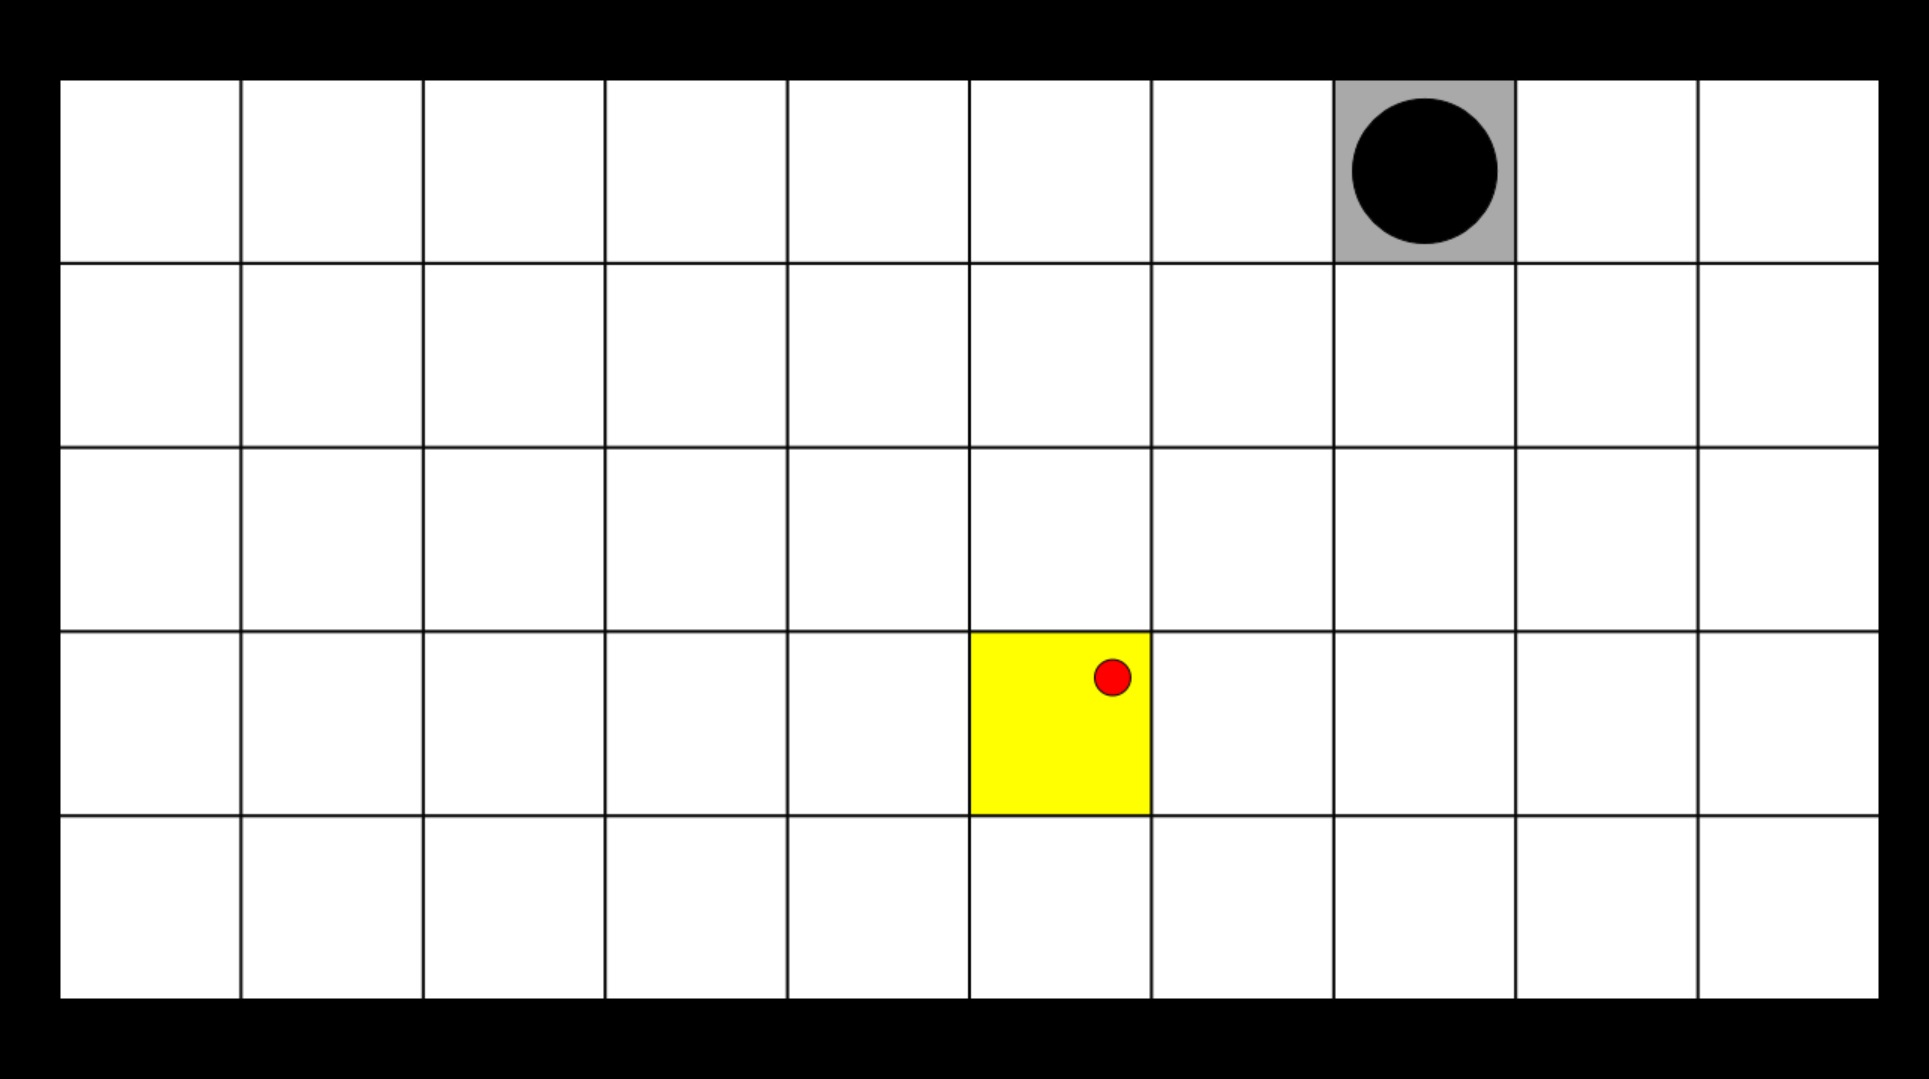
\includegraphics[width = 0.42\columnwidth , height = 2cm ]{images/kinectScreen.jpg}\label{fig:kinectScreen}} 
	\subfloat[]{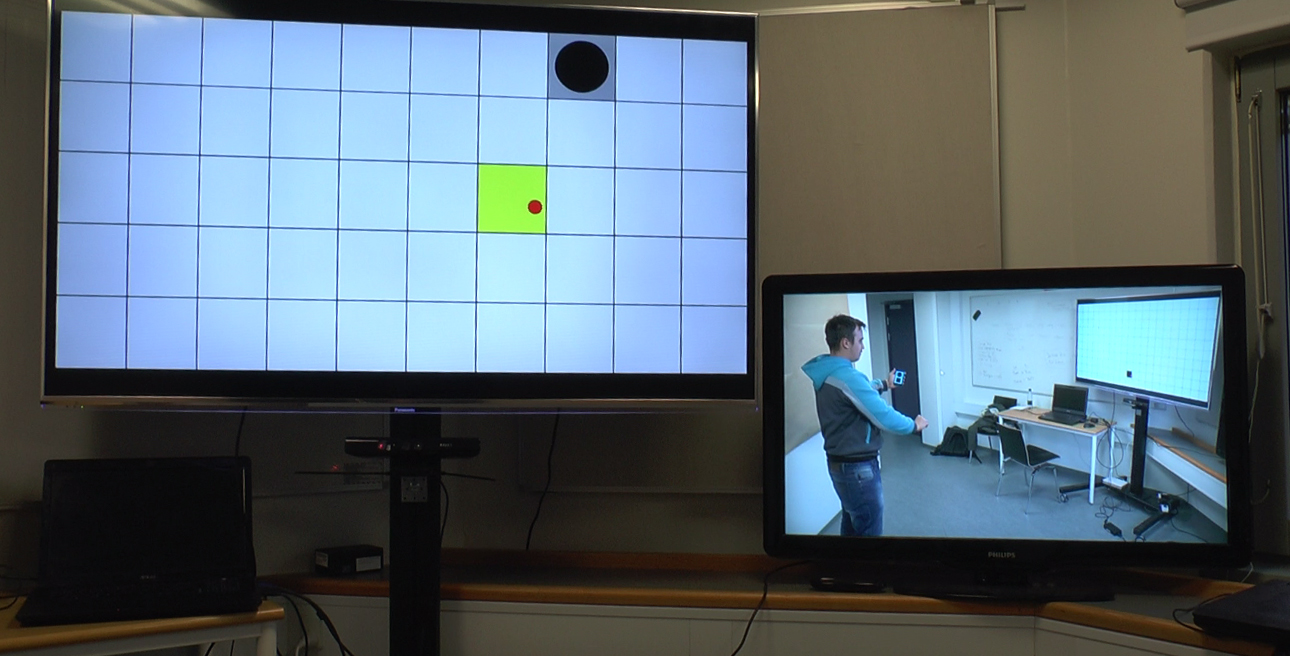
\includegraphics[width = 0.42\columnwidth , height = 2cm ]{images/setup.jpg}\label{fig:setup}}
	\subfloat[]{
\includegraphics[height = 2cm ]{images/phoneScreen.png}\label{fig:phoneScreen}} \\
	\subfloat[]{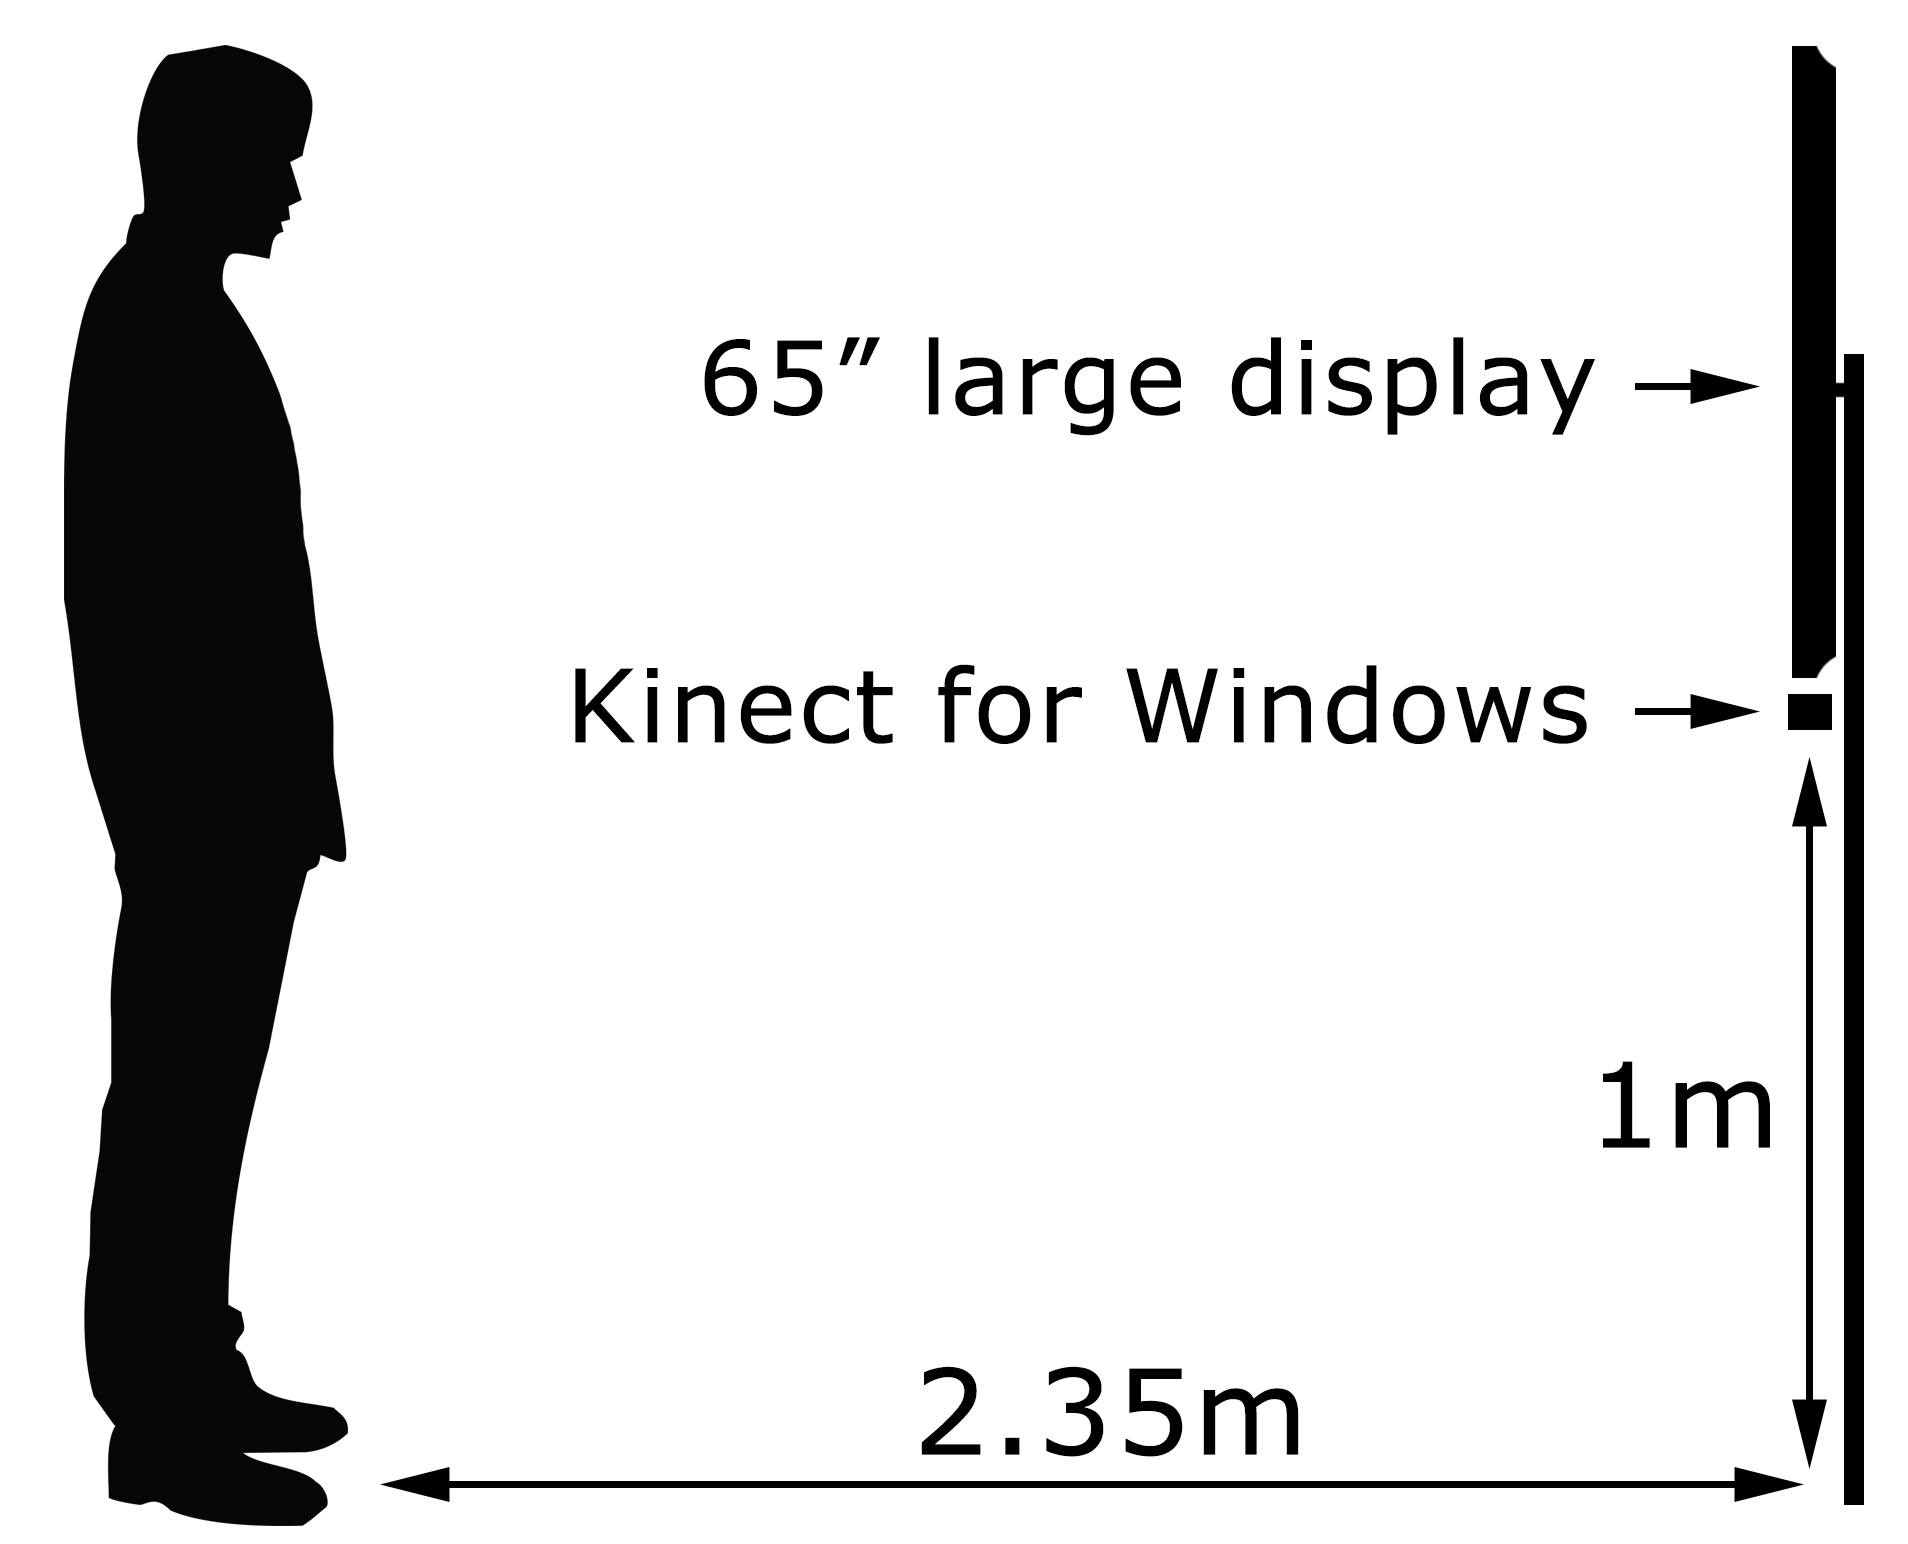
\includegraphics[width = 0.7\columnwidth]{images/SetupIllustration.jpg}\label{fig:setupDistances}}
	\caption{
		\protect\subref{fig:kinectScreen} The main screen of the application.
		\protect\subref{fig:setup} The entire setup, with the tutorial video screen on the right.
		\protect\subref{fig:phoneScreen} The phone screen showing the two shapes.
		\protect\subref{fig:setupDistances} The distance between the user and the Kinect, and the Kinect and the floor.
	}
	\label{fig:allSetup}
\end{figure}

The application would at random choose one of the four techniques and display a short explanatory movie of how to perform the technique on a screen right beside the main application display. 
A shape would appear, either a square or a circle, at one of the cells in the grid. This is the target that the participant needs to hit with the given interaction technique. This shape would be chosen at random. We chose two shapes so that it did not become a search problem. We wanted the user to spend some time orienting him or her self with the phone, but did not want them spending time searching for the correct shape. The entire setup can be seen in \Cref{fig:allSetup}.

The user would then have three practice attempts, in order to get familiar with the technique. 
For the practice phase, only the time it took the user to get through was logged and not whether targets were hit or missed. 
The user would have to choose the correct shape on the phone and perform the technique with that shape selected. 
The shapes on the phone (\cref{fig:phoneScreen}) would randomly change positions, so that the user would have to check the phone after every technique. 
The grid would also randomly, as far as the user was concerned, change size from large to small or vice-versa. In reality, the target sequences where hard coded by us in such a way that there was an equal distribution of large and small grid targets. We also made sure that there was an equal distribution of distances between each target. We classified them as short jumps, medium jumps, and long jumps. 
After the practice phase, a calibration start target would be shown. This is so that we could calculate the distance between all other targets correctly. The user would then go through the rest of the test (18 targets), going through a total of 22 targets. 

That means that our experiment had the following list of conditions:
\begin{itemize}
	 \item Technique (4)
	 \item Grid size (2)
	 \item Target jump distance (3)
	 \item Repetition (3)
\end{itemize}

This means that each user had a total of $4 \times 2 \times 3 \times 3 = 72 $ targets.

\subsection{Procedure}

Each test subject was taken into the usability lab and then given a short introduction to what we were doing and why. 
We would then explain how the system would work and what they had to do. 
We would hand them a phone, ask them to stand on a marked cross, so that the distance to the screen would always be the same, and start the test.

One of the four techniques would be chosen at random and be presented to the user. 
A short explanatory movie would be shown on a screen beside the main display showing the user how to perform the technique. 
The user would then go through the practice phase of the test, followed by the actual test. 
After that, the user would then be asked to fill in the short questionnaire regarding the technique they just tried. 

This process would be repeated four times in total, one for each technique. 
After that, we would then ask the test subject to fill in a small demographic survey. 
We asked them about their age, height, if they were left or right handed, if they had a smart phone, for how long, if they had any experience with a Kinect, Wii, Playstation Move, or any other similar air gesture based technologies, and how often they utilized them. 
We then thanked them for their time and sent them on their way. 
The entire test took on average 15 minutes. 